\documentclass[11pt,a4paper]{article}

% ---------- fonts & layout ----------
\usepackage{fontspec}
\setmainfont{LibertinusSerif}[Extension=.otf,UprightFont=*-Regular,BoldFont=*-Bold,ItalicFont=*-Italic,BoldItalicFont=*-BoldItalic]
\setsansfont{LibertinusSans}[Extension=.otf,UprightFont=*-Regular,BoldFont=*-Bold,ItalicFont=*-Italic,BoldItalicFont=*-Bold]
\setmonofont{LibertinusMono}[Extension=.otf,UprightFont=*-Regular,Scale=0.9]
\usepackage[a4paper,margin=24mm,top=22mm,bottom=24mm]{geometry}
\usepackage{microtype}
\usepackage{setspace}\setstretch{1.08}
\usepackage[english]{babel}

% ---------- figures, tables, colour ----------
\usepackage{graphicx}
\usepackage{booktabs,tabularx,array,multirow}
\usepackage{xcolor}
\definecolor{verd}{HTML}{17744F}
\definecolor{verdhi}{HTML}{3DBB82}
\definecolor{ink}{HTML}{1A1A1A}
\definecolor{dim}{HTML}{5A5F5C}
\usepackage{tikz}
\usetikzlibrary{positioning,arrows.meta,shapes.geometric,calc,fit,backgrounds}
\usepackage[font=small,labelfont={bf,sf},format=plain,labelsep=period]{caption}
\usepackage{subcaption}
\usepackage{enumitem}\setlist{nosep,leftmargin=1.4em}

% ---------- citations & links ----------
\usepackage[round,authoryear]{natbib}
\setcitestyle{aysep={}}
\usepackage[colorlinks=true,linkcolor=verd,citecolor=verd,urlcolor=verd]{hyperref}
\usepackage{doi}
\usepackage{xurl}

% ---------- section style ----------
\usepackage{titlesec}
\titleformat{\section}{\sffamily\large\bfseries}{\thesection}{0.6em}{}
\titleformat{\subsection}{\sffamily\normalsize\bfseries}{\thesubsection}{0.6em}{}
\titlespacing*{\section}{0pt}{1.1em}{0.45em}
\titlespacing*{\subsection}{0pt}{0.8em}{0.3em}

\newcommand{\grc}[1]{#1}
\newcommand{\pkm}{\textsc{Pharmakon}}

\begin{document}

% ---------- title block ----------
\begin{center}
{\sffamily\fontsize{18}{22}\selectfont\bfseries Keeping Uncertainty Visible\par}
\vspace{4pt}
{\sffamily\fontsize{12.5}{16}\selectfont A Verified, Probabilistic Reading of Dioscorides’ \textit{De materia medica},\\ from Greek Plant Names to Testable Hypotheses\par}
\vspace{10pt}
{\large Arpit}\\[2pt]
{\small National Institute of Technology Hamirpur, India}\\[6pt]
{\small\sffamily\color{dim} DH2027 · Long paper · Code, data and archive: \href{https://doi.org/10.5281/zenodo.24106413}{doi:10.5281/zenodo.24106413}}
\end{center}
\vspace{2pt}

\noindent\colorbox{verd!6}{\parbox{\dimexpr\linewidth-2\fboxsep}{\small
\textbf{\sffamily Abstract.}\enspace
Dioscorides’ \textit{De materia medica} (first century CE) is the most copied pharmacological text of the Greek tradition, but three uncertainties stand between it and testable science: which plants its names denote, which of its uses survived, and whether historical use anticipates later pharmacological research. We present \pkm{}, an open pipeline that models these uncertainties instead of resolving them by fiat. It segments Wellmann’s edition and Galen’s \textit{De simplicium medicamentorum} into CTS-addressed passages, extracts medical-use claims that must quote their Greek verbatim, assigns each ancient name a probability distribution over verified species with an explicit “unidentified” option, traces each use through Galen, John the Physician and modern ethnobotanical records, and tests predictive value in a leakage-controlled backtest. On 61 expert identifications the model’s first choice agrees 62\% of the time (95\% CI 51–75\%), against 39\% for a uniform guess and 31\% for the standard lexicon, but its probabilities are not yet calibrated. Uses recur in the modern record more often than chance (48.6\% vs.\ 40.8\%, $p = 0.001$). Historical features, however, never improve on research popularity in predicting later research, and at one cutoff make the ranking worse: we report this null as a central result. We argue that displaying contested names, untranslatable conditions and negative findings is a creative methodological choice for computational reading.
}}

\vspace{4pt}
\noindent{\small\textbf{\sffamily Keywords:} Dioscorides; Byzantine medicine; ancient Greek; uncertainty; plant identification; ethnopharmacology; reproducibility; knowledge graphs; negative results}

% ======================================================================
\section{Introduction}

The 2015 Nobel Prize in Physiology or Medicine recognised the discovery of artemisinin, a lead its discoverer found in a fourth-century Chinese handbook of emergency prescriptions \citep{tu2011}. Europe has a source of comparable reach: Dioscorides’ \textit{De materia medica}, written in the first century CE and copied, translated, excerpted and illustrated for some fifteen centuries \citep{riddle1985,leonti2011}. Its roughly six hundred plant chapters remain a reference point for Mediterranean herbal medicine \citep{leonti2017}, and quantitative surveys have catalogued thousands of therapeutic uses in its Renaissance editions \citep{staub2016}.

Turning such a text into testable hypotheses is not, however, a matter of retrieval. Three constraints intervene. First, the identity of its plants is uncertain: a single Greek name may correspond to several modern species, and authorities disagree. Second, the survival of its uses through later tradition (Galen, Byzantine compendia, living folk practice) has rarely been measured at scale. Third, the claim that historical use anticipates pharmacological activity is seldom tested in a way that excludes hindsight \citep{buenz2004}. Each constraint invites a shortcut: pick the most cited identification, count co-occurrences, or report a few successful examples. Each shortcut discards information that a historian would consider essential.

This paper presents \pkm{}, an open pipeline that treats these constraints as information to be modelled and shown. Its design rests on three commitments: every computed claim is answerable to a verbatim, citable passage; every identification is a probability distribution that may decline to name a plant; and every predictive claim is tested prospectively, with the result reported whether or not it flatters the method. The project is built for three readers at once: historians, who can read Dioscorides with evidence attached to each use; laboratories, who receive a ranked shortlist with reasons; and conservation, since each species carries its threat status where one has been assessed. The work responds to the DH2027 theme as \emph{creativity under constraint}: the fragile parts of the evidence are not cleaned away but become the product.

The paper makes four contributions: (i) a reading method in which every extracted use is a verified quotation with a stable citation; (ii) a probabilistic identification model with an explicit “unidentified” option, evaluated against published expert judgements and reported with its calibration; (iii) a measurement of how Dioscorides’ uses survive through Galen, Byzantium and the modern record, against a permutation null; and (iv) a prospective, leakage-controlled test of whether historical use anticipates later research, whose answer is negative.

% ======================================================================
\section{Background and related work}

\paragraph{Computation and ancient texts.} Machine learning for ancient languages has advanced restoration, geographical and chronological attribution, and annotation \citep{assael2022ithaca,sommerschield2023}. Open TEI editions with Canonical Text Services (CTS) citation, notably Open Greek and Latin’s First1KGreek corpus, now make Greek technical literature machine-readable and citable at the level of the passage. Pharmacological texts have received less attention than literary and epigraphic ones, even though their content (plants, preparations, conditions) links naturally to modern structured data.

\paragraph{Uncertainty as an object of study.} Philologists and historians of botany have always worked with graded certainty: commentaries on Dioscorides record competing identifications, and editors mark doubtful readings rather than suppress them. Computational pipelines, by contrast, often reduce such judgements to a single label because downstream tools expect one. Probabilistic models offer a way to keep the scholarly habit of hedging, but only if their probabilities are themselves checked: a model that says 0.7 should be right about seven times in ten. Calibration, measured here with expected calibration error \citep{naeini2015}, is therefore treated as a result in its own right rather than a technical detail.

\paragraph{Historical texts in ethnopharmacology.} Ethnopharmacologists have long argued that written traditions shape which plants are used and remembered \citep{leonti2011}. \citet{staub2016} quantified 5,314 therapeutic uses of 536 plant taxa in Matthioli’s 1568 edition of Dioscorides. Most directly relevant here, \citet{lardos2024} proposed a systematic, expert-driven methodology for assessing the identity of plants in a thirteenth-century Byzantine pharmacy text, John the Physician’s \textit{Therapeutics}, weighing botanical-historical literature, ethnobotanical evidence and lexicographic sources; their published data \citep{lardos2023data} provide the expert identifications used as our gold standard.

\paragraph{From texts to leads.} Mining historical herbals for drug leads has been advocated for two decades \citep{buenz2004}, and literature-based discovery has a longer history of proposing hidden links between disjoint bodies of knowledge \citep{swanson1986}. Two weaknesses recur. Pipelines usually commit to one identification per name, so uncertainty in the first step silently propagates to every later one. And predictive value is typically argued from retrospective examples rather than measured with a design that prevents knowledge of the future from leaking into the features \citep{kaufman2012}. \pkm{} addresses both, and connects the textual layer to open natural-products, bioactivity and disease-association resources \citep{rutz2022,zdrazil2024,buniello2025}.

% ======================================================================
\section{Sources}

Table~\ref{tab:sources} lists the corpus. The Greek texts are Wellmann’s edition of Dioscorides \citep{wellmann1907} and Galen’s \textit{De simplicium medicamentorum temperamentis ac facultatibus} in Kühn’s edition \citep{kuhn1826}, both from First1KGreek under CC BY-SA 4.0. John the Physician enters through the 61 names identified by \citet{lardos2024}. The modern record combines the ethnobotanical and herbal-medicine references compiled by Lardos et al.\ (for Greece and Cyprus) with two published Greek field surveys \citep{tsioutsiou2023,axiotis2018}. Of the 1,226 modern records, 919 come from the references compiled by Lardos et al., 241 from the North Aegean survey and 66 from Mount Pelion; the modern layer is therefore broader than village fieldwork but also less uniform in method, which the survival test inherits. Species names are verified against the GBIF backbone \citep{gbif2023}, conditions against MeSH, and compounds by InChIKey. Copyrighted modern translations are not used; translations in this paper are our own.

\begin{table}[t]
\centering\small
\caption{Corpus and reference resources. Counts are produced by the pipeline’s stage reports.}
\label{tab:sources}
\begin{tabularx}{\linewidth}{@{}l X r@{}}
\toprule
Layer & Source & Units \\
\midrule
1st c. & Dioscorides, \textit{De materia medica}, ed.\ Wellmann (TEI) & 1,500 passages, 835 chapters \\
2nd c. & Galen, \textit{De simpl.\ med.}, ed.\ Kühn (TEI) & 476 drug entries \\
13th c. & John the Physician, via \citet{lardos2024} & 61 expert-identified names \\
Modern & Lardos et al.\ references; Mount Pelion; North Aegean & 1,226 records \\
Taxonomy & GBIF backbone & 537 of 683 names verified \\
Chemistry & LOTUS, ChEMBL, Open Targets & 10,252 compounds, 455 human targets \\
Evidence & PubMed, year-stamped co-mentions & 1,999 plant–condition pairs \\
\bottomrule
\end{tabularx}
\end{table}

% ======================================================================
\section{Method}

Figure~\ref{fig:pipeline} summarises the pipeline. Every stage is a deterministic command that writes Parquet tables in which each row carries its source, retrieval time and method.

\begin{figure}[t]
\centering
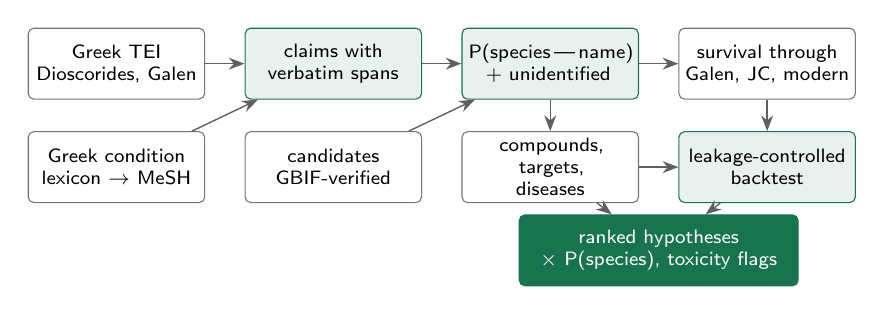
\begin{tikzpicture}[
  node distance=4mm and 5mm,
  box/.style={draw=ink!60, rounded corners=2pt, fill=white, align=center, font=\sffamily\scriptsize, minimum height=9mm, text width=21mm, inner sep=2pt},
  key/.style={box, fill=verd!10, draw=verd},
  outbox/.style={box, fill=verd, text=white, draw=verd},
  arr/.style={-{Stealth[length=2mm]}, draw=ink!70, line width=0.5pt}]
\node[box] (tei) {Greek TEI\\Dioscorides, Galen};
\node[key, right=of tei] (claims) {claims with\\verbatim spans};
\node[key, right=of claims] (id) {P(species\,|\,name)\\+ unidentified};
\node[box, right=of id] (trace) {survival through\\Galen, JC, modern};
\node[box, below=of tei] (lex) {Greek condition\\lexicon $\rightarrow$ MeSH};
\node[box, below=of claims] (cand) {candidates\\GBIF-verified};
\node[box, below=of id] (chem) {compounds, targets,\\diseases};
\node[key, below=of trace] (bt) {leakage-controlled\\backtest};
\node[outbox, below=6mm of $(chem)!0.5!(bt)$, text width=34mm] (leads) {ranked hypotheses\\$\times$ P(species), toxicity flags};
\draw[arr] (tei) -- (claims); \draw[arr] (claims) -- (id); \draw[arr] (id) -- (trace);
\draw[arr] (lex) -- (claims); \draw[arr] (cand) -- (id); \draw[arr] (id) -- (chem);
\draw[arr] (trace) -- (bt); \draw[arr] (chem) -- (bt);
\draw[arr] (bt) -- (leads); \draw[arr] (chem) -- (leads);
\end{tikzpicture}
\caption{The \pkm{} pipeline. Shaded steps carry the three methodological commitments: verbatim evidence, explicit identification uncertainty, and a prospective test. Outputs are published as a knowledge graph, a website, a JSON API and a Model Context Protocol server.}
\label{fig:pipeline}
\end{figure}

\subsection{Reading with verbatim evidence}
A rule-based extractor driven by a Greek condition lexicon proposes medical-use claims for each passage. Each claim must store the exact substring that states it, together with the passage’s CTS URN; a Unicode-normalised, whitespace-normalised substring check archives any claim whose quotation is not found, rather than silently keeping it. In this way 3,696 claims were kept with no span mismatches. Headwords were parsed for 97.6\% of chapters, and 285 chapters carry synonym lists (2,014 synonyms in total), which the pipeline keeps as alternative names rather than discarding as interpolations. Each claim also records, where the text states them, the plant part used (63\% of claims) and the route of administration (65\%). Of 158 Greek condition terms, 134 map to verified MeSH headings; 24, such as humoral states with no modern counterpart, are kept explicitly as having no modern equivalent. Language models later proposed further claims and lexicon stems under the same verification rule. These are stored separately, tagged by origin, and excluded from every evaluation reported below.

\subsection{Identification with an explicit “unidentified” option}
For each ancient name, a conditional-logit model ranks GBIF-verified candidate species. Candidates are proposed from the expert literature and the lexicon and then verified against the GBIF backbone: 537 of 683 proposed names resolved to an accepted species, while the rest (most of them names that resolve only to a genus or higher rank, a few fungi or algae) were dropped and counted rather than guessed at. Its features describe geography (occurrence in Greece and the eastern Mediterranean), continuity between the ancient name and modern Greek vernacular or Latin names, agreement among botanical-historical and ethnobotanical identifications, the lexicon’s assertion, and consensus within the candidate set’s genera; an optional feature compares Dioscorides’ description of leaves, flowers and roots with modern botanical descriptions. Crucially, “unidentified” is a candidate with its own learned utility, so a name with thin evidence receives a high probability of remaining unidentified instead of a forced answer. Predictions are temperature-scaled and reported with bootstrap intervals (Appendix, Table~\ref{tab:weights}).

\subsection{Tracing survival}
Each name–use pair is followed through Galen, John the Physician and the modern record and classified as persisted, persisted only as far as Galen or Byzantium, modified, or lost. Galen’s entries are aligned to Dioscorides’ chapters through their headwords and synonyms: 339 of the 476 entries map to a Dioscorides chapter, and the remaining 137 are reported as unmapped rather than forced. Because later authors copy earlier ones, Galen entries whose wording overlaps the matched Dioscorides chapter (word 4-gram containment above 0.15) are down-weighted; in practice containment was low (mean 0.002), so the agreement is not textual copying. Observed survival is compared with a permutation null that shuffles the use labels of the modern records while keeping their plants fixed, so that the overall frequency of each use is preserved.

\subsection{A prospective test}
To ask whether history anticipates later research, a rolling-origin backtest stands at 2000, 2005, 2010 and 2015. At each cutoff it ranks plant–condition pairs not yet studied, using only information dated on or before the cutoff (compound reference years, bioactivity document years and modern-study publication years are all gated by date), and scores the ranking against PubMed pharmacology co-mentions that appeared afterwards, up to 2025. At each cutoff a logistic model is fitted on pairs observable before the cutoff and applied to the unstudied pairs; models with history features are compared with research popularity alone, chemistry, a shuffled-history control and a combined model. No language-model output enters this test, and the identification step it relies on uses no pharmacology.

\subsection{Hypotheses and their paths}
Untested pairs are ranked by the forecast score weighted by the probability that the plant is correctly identified, and linked through a knowledge graph of 2,585 nodes and 9,146 edges to compounds, human protein targets and diseases (Figure~\ref{fig:path}). Toxic genera carry a hazard citation, and the flag is displayed rather than filtered. The same records are served to people through a website and to AI assistants through a Model Context Protocol server.

\begin{figure}[t]
\centering
\resizebox{\linewidth}{!}{%
\begin{tikzpicture}[
  node distance=3.2mm,
  hop/.style={draw=verd, rounded corners=2pt, fill=verd!7, align=center, font=\sffamily\scriptsize, minimum height=11mm, text width=19.5mm, inner sep=2pt},
  arr/.style={-{Stealth[length=1.8mm]}, draw=verd, line width=0.6pt},
  lab/.style={font=\sffamily\tiny, text=dim, above, midway}]
\node[hop] (a) {Passage 2.105.2\\{\rmfamily\small ὀφθαλμῶν προπτώσεις}\\eye prolapse};
\node[hop, right=of a] (b) {ancient name\\{\rmfamily\small κύαμος}};
\node[hop, right=of b] (c) {\textit{Vicia faba}\\P = 0.66\\{[0.51, 0.81]}};
\node[hop, right=of c] (d) {naringenin\\CHEMBL9352};
\node[hop, right=of d] (e) {CA4\\pChEMBL 7.1};
\node[hop, right=of e] (f) {retinitis\\pigmentosa\\OT score 0.67};
\draw[arr] (a) -- node[lab]{mentions} (b);
\draw[arr] (b) -- node[lab]{identified as} (c);
\draw[arr] (c) -- node[lab]{contains} (d);
\draw[arr] (d) -- node[lab]{acts on} (e);
\draw[arr] (e) -- node[lab]{associated} (f);
\end{tikzpicture}}
\caption{One hypothesis as a path through the knowledge graph (top-ranked lead, eye diseases; no known toxicity). Every hop carries its source, so the lead traces back to the words Dioscorides wrote. A path is a reason to test, not evidence of effect.}
\label{fig:path}
\end{figure}

% ======================================================================
\section{A worked example: \grc{ἀψίνθιον}}

In chapter 3.23 Dioscorides writes: \textit{\grc{δύναμιν δὲ ἔχει στυπτικήν, θερμαντικήν, ἀποκαθαρτικὴν τῶν ἐνηρεικότων στομάχῳ καὶ κοιλίᾳ χολωδῶν}} (“it has an astringent, warming power, purging the bilious matter lodged in the stomach and belly”). The pipeline extracts each use with its span and URN (\nolinkurl{urn:cts:greekLit:tlg0656.tlg001.1st1K-grc1:3.23.1}). For the name it assigns \textit{Artemisia absinthium} a probability of 0.75 (90\% interval 0.62–0.88), leaves 0.23 to “unidentified”, and 0.02 to \textit{A.\ monosperma} (Figure~\ref{fig:example}a). Of its twelve use groups, the skin and wound uses are attested in Galen and expected in the modern record, while most others are not (Figure~\ref{fig:example}b). The 0.23 assigned to “unidentified” is not a failure but a statement about the evidence: the name is well known, yet the description and the later tradition leave room for another wormwood. The reader sees not a verdict but a weighted reading, with the evidence for each weight one click away.

\begin{figure}[t]
\centering
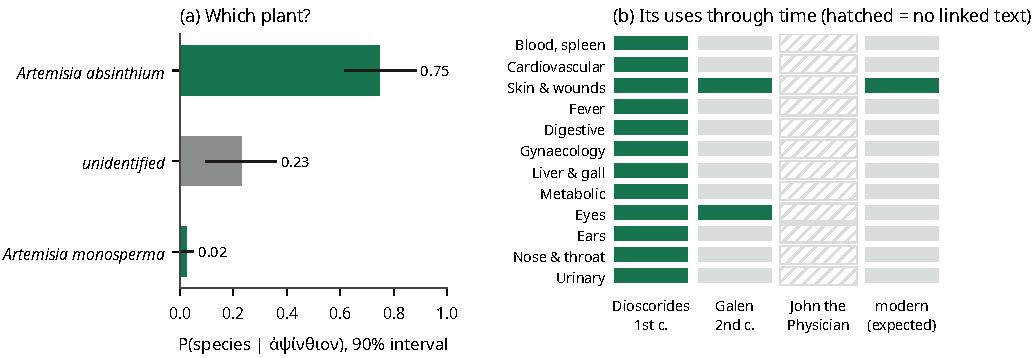
\includegraphics[width=\linewidth]{figures/fig_example.pdf}
\caption{Worked example for \grc{ἀψίνθιον} (\textit{De materia medica} 3.23). (a) Probability over candidate species with 90\% bootstrap intervals, including the explicit “unidentified” option. (b) Survival of each use group across eras; John the Physician does not treat this name in the expert sample.}
\label{fig:example}
\end{figure}

% ======================================================================
\section{Results}

\subsection{Which plant is it?}
Holding out each expert name in turn, the model’s first choice matches the expert identification for 62\% of the 61 names (95\% CI 51–75\%; Figure~\ref{fig:ident}a, Table~\ref{tab:results}); the expert answer is among the model’s top three for 92\%, and the mean reciprocal rank is 0.78. The baselines set this in proportion. Candidate lists are short (141 candidates for 61 names, drawn from the same expert study), so a uniform guess already reaches 39\% and a genus-frequency prior 38\%. The lexicon’s single identification reaches only 31\%, below chance. Two features overlap the experts’ own evidence; a transfer model trained without them reaches 56\%, the cleanest estimate. A language model given the Greek and the candidate list reaches 59\%, but may have memorised the literature and is reported for comparison only. Agreement tracks the experts’ own confidence: 68\% where they rated the identification strong, 73\% for moderate, and 13\% for the eight names they rated weak. Ablations show where the agreement comes from (Appendix, Table~\ref{tab:weights}). Removing scholarly agreement lowers top-1 agreement to 54\%, whereas removing geography raises it slightly, to 66\%, at the cost of worse calibration (ECE 0.24); with 61 names these differences lie within the intervals and should be read as tendencies. Calibration misses its target: expected calibration error \citep{naeini2015} is 0.14 before temperature scaling and 0.21 after, against a target of 0.10 (Figure~\ref{fig:ident}b).

\begin{figure}[t]
\centering
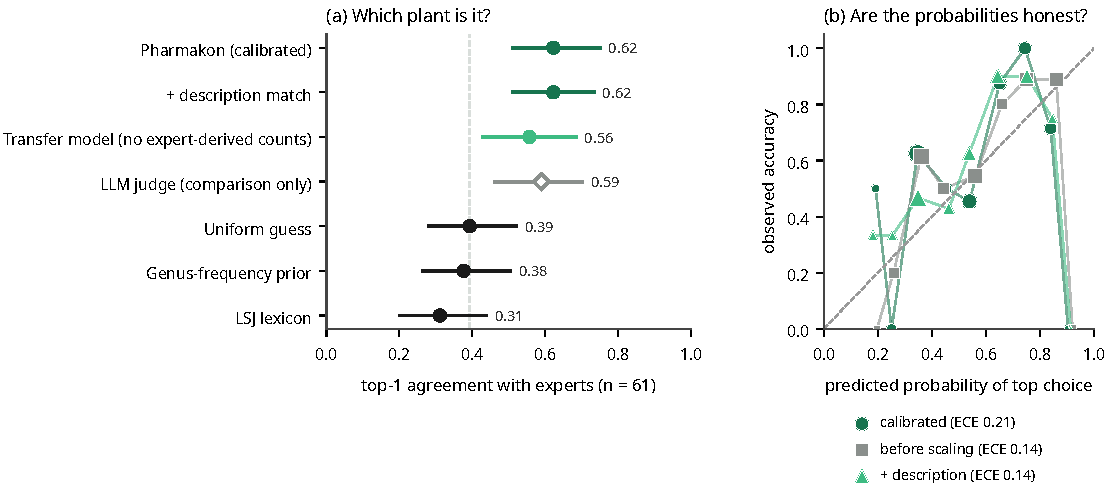
\includegraphics[width=\linewidth]{figures/fig_identification.pdf}
\caption{Identification against 61 expert names. (a) Top-1 agreement with 95\% bootstrap intervals; the dashed line marks a uniform guess. (b) Reliability diagram; marker area is proportional to the number of names in each bin, and the diagonal is perfect calibration.}
\label{fig:ident}
\end{figure}

\subsection{Did the uses survive?}
Of 1,533 name–use rows, 247 persist to the modern record, 130 reach Galen but no further, 261 are modified and 499 are lost (Figure~\ref{fig:survival}). Restricting to the 508 rows whose plant is attested in the modern record, 48.6\% of uses recur, against 40.8\% under 1,000 permutations (95th percentile 43.3\%; $p = 0.001$). A further 387 uses appear in later sources for the same plants without a precedent in Dioscorides, a reminder that the tradition also innovated. Skin and wound uses dominate both the corpus and the survivors; one of the modern surveys concerns skin ailments only, which favours this group slightly.

\begin{figure}[t]
\centering
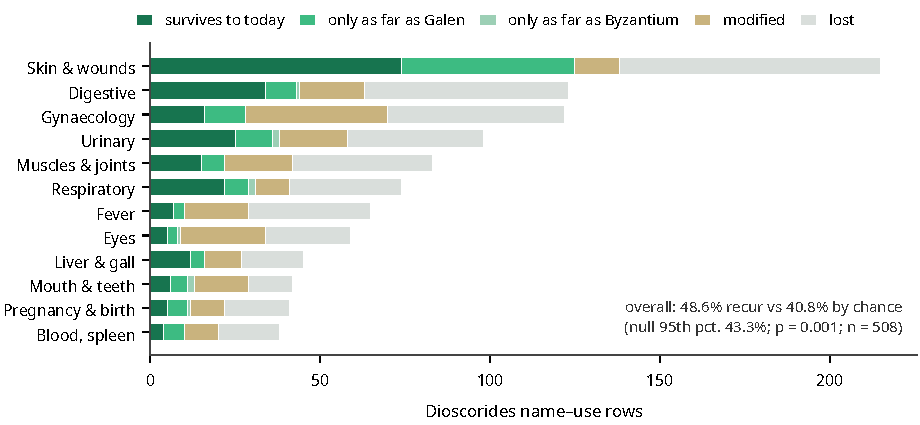
\includegraphics[width=\linewidth]{figures/fig_survival.pdf}
\caption{What happened to Dioscorides’ uses, by body system (twelve largest groups). Rows are name–use pairs; “modified” uses recur with a changed indication or preparation.}
\label{fig:survival}
\end{figure}

\subsection{Does history predict later research?}
It does not (Figure~\ref{fig:backtest}). Research popularity alone (the number of earlier PubMed records on the species and on the condition) reaches an area under the precision–recall curve of 0.27–0.38 across cutoffs, four to seven times the random baseline. Adding the historical features never improves on it; at the 2005 cutoff it makes the ranking worse ($\Delta$AUPRC $-0.14$ to $-0.02$, 95\% CI), and at the other cutoffs the interval includes zero. At 2005 the bootstrap places 99.7\% of its mass at or below zero for the gain from history, while popularity alone reaches an area under the ROC curve of 0.86. History alone performs close to random, and a shuffled-history control, which should carry no signal, scores within a few points of the real historical features. Chemistry carries some signal but adds nothing beyond popularity (Appendix, Table~\ref{tab:backtest}).

\begin{figure}[t]
\centering
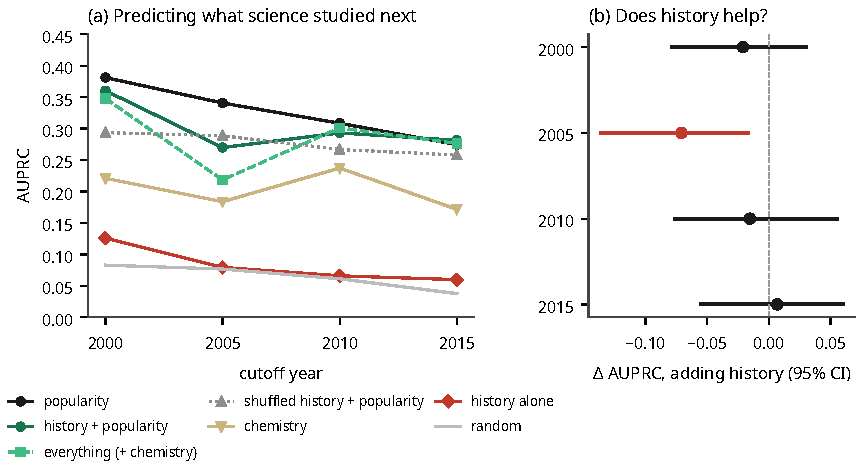
\includegraphics[width=\linewidth]{figures/fig_backtest.pdf}
\caption{Rolling-origin backtest across all body systems. (a) AUPRC by cutoff for each feature set. (b) Change in AUPRC when historical features are added to popularity, with 95\% bootstrap intervals; red marks an interval entirely below zero.}
\label{fig:backtest}
\end{figure}

\subsection{What the language-model layer added}
Language models were used only as proposers, and none of their output enters the backtest. A model read 1,158 passages and proposed 5,075 claims; every one carried a Greek span that passed the substring check, it recovered 94.9\% of the rule-extracted uses, and it confirmed 468 of the 614 claims the rules had marked as ambiguous. The number of usable claims rose from 2,561 to 3,550, and 1,616 proposals fell outside the lexicon and are held apart as candidate lexicon entries for human review. The same verification rule applied to plant descriptions, which supply the description-match feature. The design point is that a language model can widen coverage without becoming an authority: its proposals are kept, labelled and checked, never trusted.

\subsection{What can be tested}
Weighting each untested pair by the probability of its plant yields 1,781 research hypotheses. Ignoring identification uncertainty would change 5 of the top 20, which is the practical cost of the shortcut described in the introduction; over the full ranking, the weighted and unweighted orders agree only moderately (Kendall’s $\tau = 0.50$). Only two of the top 20 rest on a plant whose identification probability is below 0.5, and those are flagged as such. Sixteen of the top 20 have a complete compound–target–disease path; seven carry a toxicity flag.

\begin{table}[t]
\centering\small
\caption{Summary of results. All figures are produced by the pipeline’s stage reports.}
\label{tab:results}
\begin{tabularx}{\linewidth}{@{}X l r l@{}}
\toprule
Question & Measure & Result & Comparison \\
\midrule
Which plant is it? & top-1 agreement, $n = 61$ & 0.62 [0.51, 0.75] & uniform 0.39; lexicon 0.31; transfer 0.56 \\
Are the probabilities honest? & expected calibration error & 0.14–0.21 & target $\le 0.10$ (not met) \\
Did the uses survive? & share recurring, $n = 508$ & 0.486 & null 0.408; $p = 0.001$ \\
Does history predict research? & $\Delta$AUPRC vs popularity & no gain & 2005: $-0.14$ to $-0.02$ \\
What can be tested? & untested plant–condition pairs & 1,781 & 16/20 with path; 7/20 toxic \\
\bottomrule
\end{tabularx}
\end{table}

% ======================================================================
\section{Discussion}

\paragraph{Creativity under constraint.} The project’s central design choice is to display what is fragile: names the experts dispute, conditions that do not map onto modern medicine, and a prediction test that failed. Verbatim spans and CTS URNs keep every computed claim answerable to a passage a philologist can check. The “unidentified” option allows the model to decline, which is how a careful scholar reads a contested name. And the null result is informative in its own right: under a design that blocks hindsight, the historical record did not anticipate which plant–condition pairs modern pharmacology would study. Anecdotes such as artemisinin are real, but they do not show that historical use is a general predictor; evaluations that report only successes should be read with that in mind.

\paragraph{Reading the null.} Several explanations are compatible with the negative backtest, and they matter for how the result should be used. Modern research attention follows funding, existing literature and available assays, so popularity is a strong predictor almost by construction, and historical salience may simply be uncorrelated with what laboratories choose to study. The label itself is a proxy: a PubMed co-mention records that a plant and a condition were studied together, not that the plant worked. And positives are sparse (50 to 122 per cutoff), so moderate effects could escape detection. The result therefore does not show that ancient knowledge is pharmacologically empty; it shows that, measured this way, it does not tell us what science will study next, and that claims to the contrary need comparably strict tests.

\paragraph{What digital humanities gains.} For computational reading, the pipeline offers a template in which machine-made claims remain citable passages, uncertainty is a first-class output, and negative results are publishable outputs rather than failures. The same records serve a historian reading Dioscorides, a laboratory choosing what to test, and an AI assistant answering questions, which encourages consistent provenance across audiences.

\paragraph{Infrastructure and responsibility.} Publishing the records through a Model Context Protocol server means that AI assistants answer questions about Dioscorides from the same verified tables, with the same uncertainty and toxicity flags, rather than from memory. The system displays no dosing; quantities appear only inside quoted historical text. Toxic genera carry a hazard citation, and every response repeats that the outputs are research hypotheses. Modern ethnobotanical data are used only at the aggregate level of published tables, and any commercial follow-up of folk knowledge falls under access-and-benefit-sharing obligations.

\paragraph{Limitations.} Expert judgement is not ground truth, and with 61 names the intervals are wide. Candidate lists and two features derive from the same expert study, which the transfer model only partly mitigates. A PubMed co-mention is a proxy for evidence, not a finding, and its precision has not yet been audited. Extraction, condition mapping and labels await blinded human audits. The Byzantine chain lacks Paul of Aegina, and John the Physician is reached only through the expert sample. Open Targets associations are current rather than historical, so a model without them is also reported. All outputs are research hypotheses, not medical advice.

% ======================================================================
\section{Conclusion}

\pkm{} shows that a classical pharmacological text can be read computationally without hiding what is uncertain. The identification step agrees with experts well above chance while declining to guess where evidence is thin; the survival of uses into the modern record exceeds chance; and the hypothesis that history predicts later research does not survive a prospective test. Because every number in this paper is regenerated by one command from open sources, the analysis can be rerun, extended to other texts, or challenged in detail. Next steps are blinded expert audits, richer plant descriptions, further Byzantine authors, Arabic and Latin transmission, and a partnership with a pharmacognosy laboratory to test the highest-ranked non-toxic hypotheses.

% ======================================================================
\section*{Data and code availability}
\small
All code, processed tables and figures are open under the MIT licence (data under each source’s licence): \url{https://github.com/LSUDOKO/Pharmakon}, archived at \doi{10.5281/zenodo.24106413} \citep{arpit2026pharmakon}. A live explorer, JSON API and MCP server run at \url{https://pharmakon.adoranto737.workers.dev}.

\section*{Disclosure of generative AI use}
\small
\textit{Research.} Two language models, Claude (Anthropic) and gpt-oss-120b (via Groq), were used to propose additional medical-use claims and condition-lexicon stems, to extract plant-description traits, and as a comparison baseline (“LLM judge”). Every proposed claim and trait had to quote its source verbatim and was kept only if the quotation was found by exact string match; all language-model outputs are excluded from the backtest. Claude Code was used extensively to write the software, documentation and website. \textit{Submission.} This paper was drafted with the assistance of Claude and was reviewed, edited and approved by the author, who takes full responsibility for its content.

\normalsize
\bibliographystyle{abbrvnat}
\bibliography{refs}

% ======================================================================
\clearpage
\appendix
\section*{Appendix}
\renewcommand{\thetable}{A\arabic{table}}\setcounter{table}{0}

\begin{table}[h]
\centering\small
\caption{Conditional-logit weights of the identification model (standardised features). The “unidentified” option has utility $-0.40$; temperature $T = 1.20$.}
\label{tab:weights}
\begin{tabularx}{\linewidth}{@{}l X r@{}}
\toprule
Feature & What it measures & Weight \\
\midrule
Present in Greece & at least one GBIF occurrence in Greece & 0.69 \\
Botanical-history support & references proposing the taxon for the name & 0.47 \\
Ethnobotanical support & references linking the name to the taxon & 0.35 \\
Regional occurrences & log GBIF occurrences in Greece, Cyprus, Turkey & 0.22 \\
Description match & agreement of Dioscorides’ description with a modern one & 0.18 \\
Genus consensus & share of candidates in the same genus & 0.18 \\
Latin-name similarity & similarity of the Latinised name to genus or epithet & 0.08 \\
Vernacular similarity & similarity to modern Greek vernacular names & 0.03 \\
Lexicon assertion & the lexicon gives this binomial & $-0.29$ \\
\bottomrule
\end{tabularx}
\end{table}

\begin{table}[h]
\centering\small
\caption{Rolling-origin backtest across all body systems: AUPRC by feature set. Positives are untested pairs that gained PubMed pharmacology support by 2025. No language-model output is used.}
\label{tab:backtest}
\begin{tabular}{@{}rrrrrrrrr@{}}
\toprule
Cutoff & Pairs & Positives & Random & Popularity & History & Chemistry & Hist.\,+\,pop. & $\Delta$ [95\% CI] \\
\midrule
2000 & 1,404 & 122 & 0.08 & 0.38 & 0.13 & 0.22 & 0.36 & $-0.08$ to $+0.03$ \\
2005 & 1,384 & 102 & 0.08 & 0.34 & 0.08 & 0.18 & 0.27 & $-0.14$ to $-0.02$ \\
2010 & 1,361 & 79 & 0.06 & 0.31 & 0.07 & 0.24 & 0.29 & $-0.08$ to $+0.06$ \\
2015 & 1,332 & 50 & 0.04 & 0.27 & 0.06 & 0.17 & 0.28 & $-0.05$ to $+0.06$ \\
\bottomrule
\end{tabular}
\end{table}

\end{document}
